\documentclass[tikz,border=10pt]{standalone}
\usepackage{pgfplots}
\usepgfplotslibrary{groupplots}
\pgfplotsset{compat=1.18}

\begin{document}
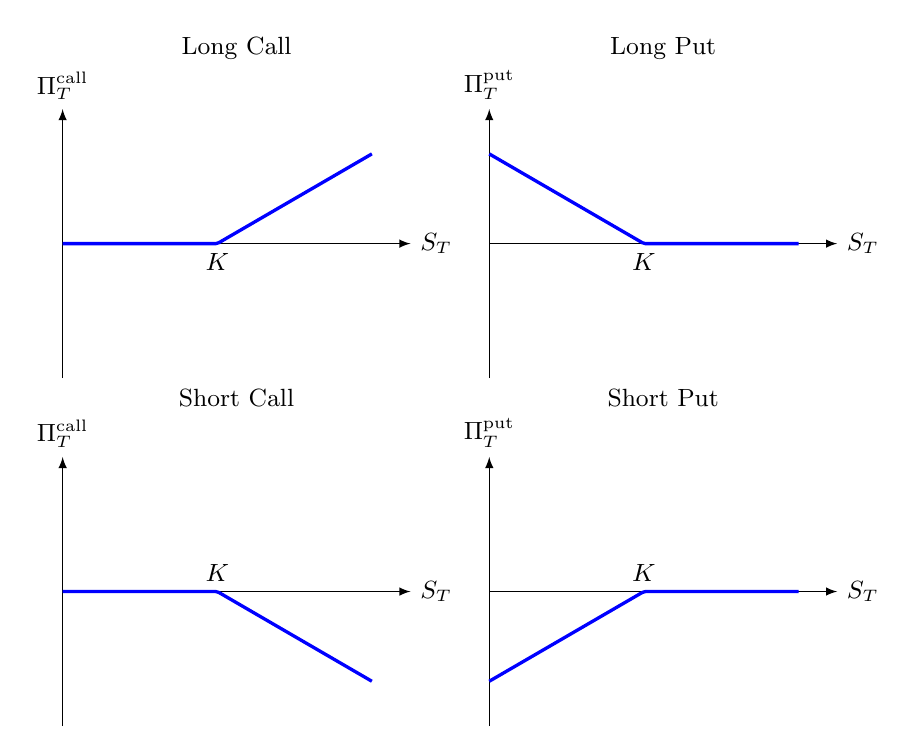
\begin{tikzpicture}[font=\small]

  \pgfmathsetmacro{\K}{2}

  \begin{groupplot}[
      group style={
          group size=2 by 2,
          horizontal sep=1cm,
          vertical sep=1cm,
        },
      width=6cm, height=5cm,
      axis lines=middle,
      axis line style={-latex},
      xmin=0, xmax=4.5,
      ymin=-3, ymax=3,
      xtick=\empty, ytick=\empty,
      domain=0:4,
      samples=100,
      every axis plot/.style={blue, very thick, no marks},
      xlabel={$S_T$},
      xlabel style={at={(axis description cs:1,0.5)}, anchor=west},
      title style={
          at={(axis description cs:0.5,1)},
          yshift=0.3cm,
          anchor=south,
        },
      clip=false,
    ]

    % Long Call
    \nextgroupplot[
      ylabel={$\Pi_T^\mathrm{call}$},
      ylabel style={at={(axis description cs:0,1)}, anchor=south},
      title={Long Call},
    ]
    \addplot {max(x-\K,0)};
    \draw (axis cs:\K,0) node[below] {$K$};

    % Long Put
    \nextgroupplot[
      ylabel={$\Pi_T^\mathrm{put}$},
      ylabel style={at={(axis description cs:0,1)}, anchor=south},
      title={Long Put},
    ]
    \addplot {max(\K-x,0)};
    \draw (axis cs:\K,0) node[below] {$K$};

    % Short Call
    \nextgroupplot[
      ylabel={$\Pi_T^\mathrm{call}$},
      ylabel style={at={(axis description cs:0,1)}, anchor=south},
      title={Short Call},
    ]
    \addplot {-max(x-\K,0)};
    \draw (axis cs:\K,0) node[above] {$K$};

    % Short Put
    \nextgroupplot[
      ylabel={$\Pi_T^\mathrm{put}$},
      ylabel style={at={(axis description cs:0,1)}, anchor=south},
      title={Short Put},
    ]
    \addplot {-max(\K-x,0)};
    \draw (axis cs:\K,0) node[above] {$K$};

  \end{groupplot}
\end{tikzpicture}
\end{document}
